


We are seeking numerical methods which, when synthesized and simulated on a quantum device, undergo a speedup relative to the original design implemented on a standard electronic computer. To this end we have discussed several potential methods that could take advantage of the design of a quantum computer. they are listed in a table below: 

\begin{center}
\begin{tabular}{|c|c|}
\hline
Algorithm&Description\\ 
\hline 
High-Dimensional Numerical Integration&\\ 
\hline
Combinatorial Optimization&\\
\hline
\end{tabular}
\end{center}

We also plan to take advantage of previous work in the realm of quantum summation and integration \cite{Traub:2002}. Although we will make use of these quantum algorithms in our research, the real utility of this project is seen in the next section where previous work by the authors will be discussed. 

The problem itself is extremely practical as we are entering the age of big data, where these numerical methods need to be implemented in more efficient ways to balance increasing data set sizes. A prerequisite to constructing numerical algorithms for quantum computers is access to, or emulation of, a quantum computer. While we do not have direct access to a quantum computer, and the emulation of a quantum computer is a challenge in itself, in the next section we discuss our previous work in constructing a quantum computer emulation and programming environment that will address this challenge.

    %\begin{figure} [h!]
      %  \centering
     %   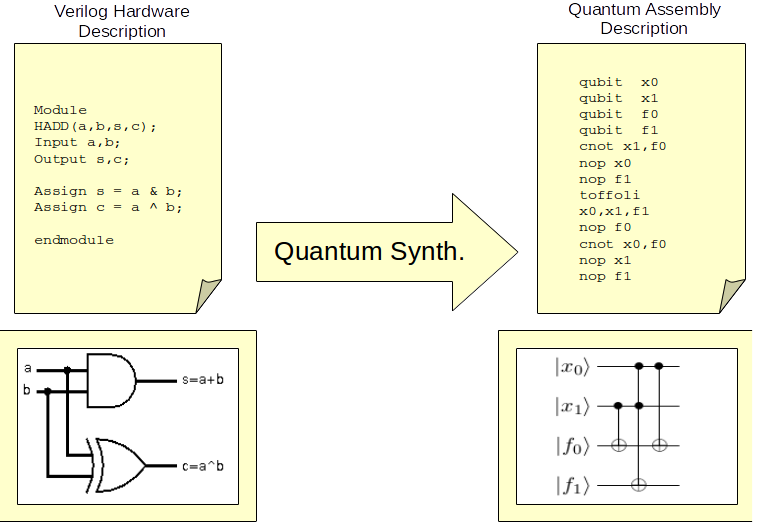
\includegraphics[scale = 0.35]{QuantumSynthesis.png}
    %\end{figure}

